\chapterimage{pi-cluster.jpg} % Chapter heading image

\chapter{Pi Cluster Form Factor}\label{c:pi-cluster-form-factor}


In this chapter we will discuss a number of opportunities to build
small scale compute and cluster resources using Raspberry Pi's.

This includes the following:

\begin{itemize}

\item a NAS server with one Raspberry Pi 3 (Section~\ref{nas-1-pi})

\item a Cluster using 1 Raspberry Pi as master and 4 Raspberry Zeros
  as workers (Section~\ref{clusterhat-4-zero-1-pi})

\item a Cluster with 5 Raspberry Pi's (Section
 ~\ref{S:cluster-case-with-cooling-5-pi}). A minimum of 3 is needed.

\item a Cluster with 40 Raspberry Pi's (Section
 ~\ref{bitscope-case-40-pi})

\item a Cluster with 144 Raspberry Pi's (Section
 ~\ref{bitscope-cluster-144-pi})

\item our recommended 5 node Raspberry Pi Cluster (Section
 ~\ref{s:pi5}). 3 nodes need to be used at minimum.
 

\end{itemize}

\section{NAS (1 Pi)}\label{nas-1-pi}

Although a NAS is not really a compute cluster the Pi has used many
times to build a Network Attached Storage (NAS) server. In this
configuration a HDD is attached to the Raspberry and the network
features of the Raspberry is used to access the disk drive via
software installed on the PI that make this easily possible. Many
tutorials exists on the Web that help setting op such a device.

We like to hear from you if you have successfully developed such a NAS
and provide us with such links. Links that may help include:

  \URL{https://hackmypi.com/NASpi.php}


\section{ClusterHat (4 Zero + 1 Pi)}\label{clusterhat-4-zero-1-pi}

The smallest cluster we came across is actually a hybrid cluster in
which 4 Pi zeros attached to a Raspberry Pi 3. Thi sis achieved via an
add on board to the Pi 3 allowing to plug in PI=i Zeros:


  \URL{https://clusterhat.com/}


The Cluster HAT (Hardware Attached on Top) allows to attach 4 Raspberry
Pi Zeros via to be attached to a regular Raspberry PI 3 to simulate a
small cluster.

According to the Web Site it supports the following features:



\begin{itemize}
\item
  USB Gadget Mode: Ethernet and Serial Console.
\item
  Onboard 4 port USB 2.0 hub.
\item
  Raspberry Pi Zeros powered via Controller Pi GPIO (USB optional).
\item
  Individual Raspberry Pi Zero power controlled via * Controller Pi GPIO
  (I2C).
\item
  Connector for Controller Serial Console (FTDI Basic).
\item
  Controller Pi can be rebooted without interrupting power to Pi Zeros
  (network recovers on boot).
\end{itemize}

\begin{figure}
\centering
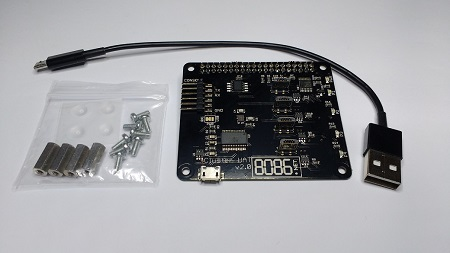
\includegraphics[width=0.5\textwidth]{images/ClusterHAT-v2-supplied-sm.jpg}
\caption{clusterhat}
\end{figure}



Links:


\URL{https://www.raspberrypi.org/magpi/clusterhat-review-cluster-hat-kit/}{clusterhat
  on raspberrypi.org}


Although this setup seems rather appealing, the issue is with obtaining
Pi Zeros for the regional price of \$5. Typically users can only by one
for that price and must pay shipping. To by more one has to buy a kit
for about \$20. However, for that amount of money it may just be worth
while to get Pi 3's instead of zero's. Nevertheless the formfactor is
rather appealing.

\section{Cluster Case With Cooling (5 Pi)}\label{S:cluster-case-with-cooling-5-pi}

Many instructions on the Web exist describing how to build clusters with
3 or more Pi's. One of the considerations that we have to think about is
that we may run rather demanding applications on such clusters causing
heat issues. To eliminate them we must provide proper cooling. In some
cluster projects cooling is not adequately addressed. Hence we like to
provide an example that discusses in detail how to add a fan and what the
fan has for an impact on the temperature.

\begin{figure}
\centering
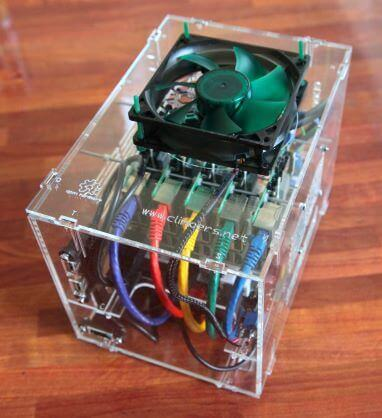
\includegraphics[width=0.5\textwidth]{images/IMG16_6273_sweb.jpg}
\caption{}
\end{figure}


\URL{http://climbers.net/sbc/add-fan-raspberry-pi/}

\URL{http://climbers.net/sbc/diy-raspberry-pi-3-cluster/}


From the above Web page we find the following information as shown in
Table~\ref{F:pi-fan}. From the data in the table it is clear that we
need to keep the Pi from throttling while being in a case by adding a
fan as obvious from experiment No. 2.



\begin{table}[htb]
\caption{Temperature comparision of fan impact}\label{F:pi-fan}
\bigskip
\begin{center}
\begin{tabular}{llllllll}
\hline
No. & Case & Fan & Direction & RPM & Idle & 100\% Load &
Performance\tabularnewline
\hline
1 & no & no & - & - & 41.0C & 75.5C & OK (barely)\tabularnewline
2 & yes & no & - & - & 45.0C & 82.5C & throttles\tabularnewline
3 & yes & 5V & in & unkown & 37.9C & 74.5C & OK (barely)\tabularnewline
4 & yes & 7V & in & 800 & 35.6C & 69.5C & OK\tabularnewline
5 & yes & 12V & in & 1400 & 32.5C & 61.1C & OK\tabularnewline
6 & yes & 7V & out & 800 & 34.5C & 66.4C & OK\tabularnewline
\hline
\end{tabular}
\end{center}
\end{table}




\section{Bitscope Case (40 Pi)}\label{bitscope-case-40-pi}

A company from Australia called BitScope Designs offers a number of
cases that leverage their Pi Blade boards allowing up to four Pis to be
put together and sharing the same power supply. The blades are shown in
Figure b.1. The rack to place 10 of them is shown in Figure b.2.

\begin{figure}
\centering
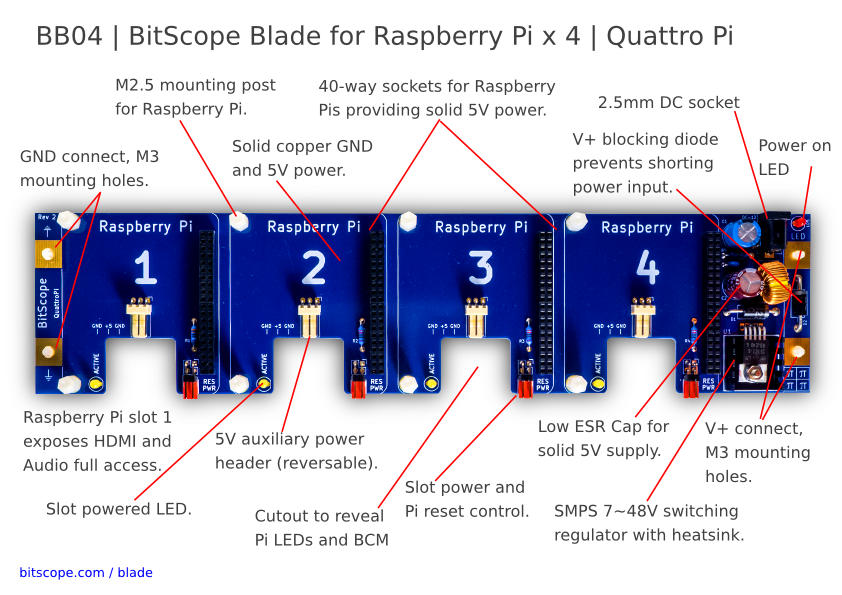
\includegraphics[width=0.3\textwidth]{images/04.jpg}
\caption{Bitscope blade for 4 Pi's.}
\end{figure}


\begin{figure}
\centering
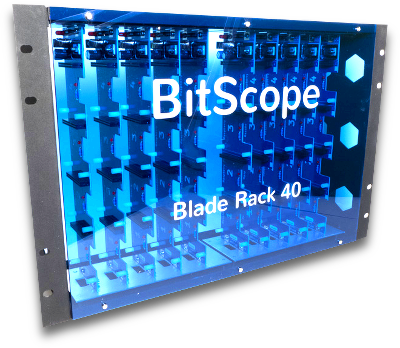
\includegraphics[width=0.3\textwidth]{images/br40a.png}
\caption{40 Pi Blade rack.}
\end{figure}


The cost of the balde rack is \$ 795.45 + \$60.00 shipping + import tax.
This may originally sound expensive when compared to a single case,
however as we can store 40 Pis in them and they can share the
power-supply and reduce cabeling we think this case is quite interesting
overall due to its price-point of \$20 per Pi.



\section{Bitscope Cluster (144 Pi)}\label{bitscope-cluster-144-pi}

https://www.youtube.com/watch?v=78H-4KqVvrg

Together with LANL a new cluster module that holds 144 Pis is developed.
This sytem is targeted to be placed into a rack to create a large Pi
cluster. The cost for such a module is about \$15K. Figure
\ref{F:pi-mod-1} shows the
module and Figure~\ref{F:pi-mod-2} shows how multiple modules can be placed into a
single rack.

\begin{figure}
\centering
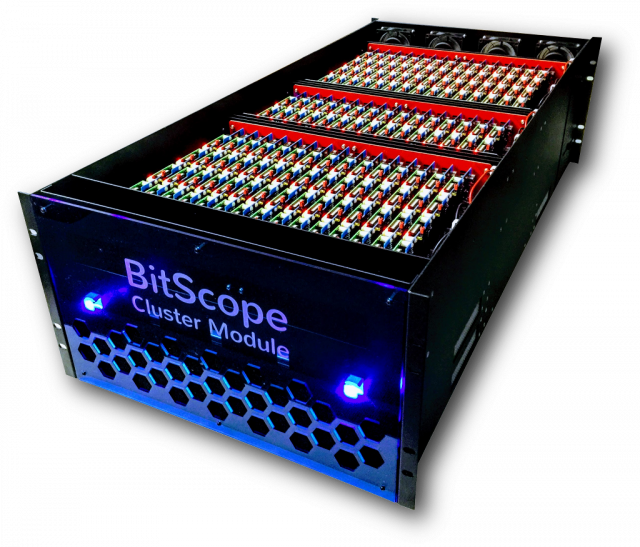
\includegraphics[width=0.5\textwidth]{images/cluster-module.png}
\caption{Bitscope 144 cluster module.}\label{F:pi-mod-1}
\end{figure}

\begin{figure}
\centering
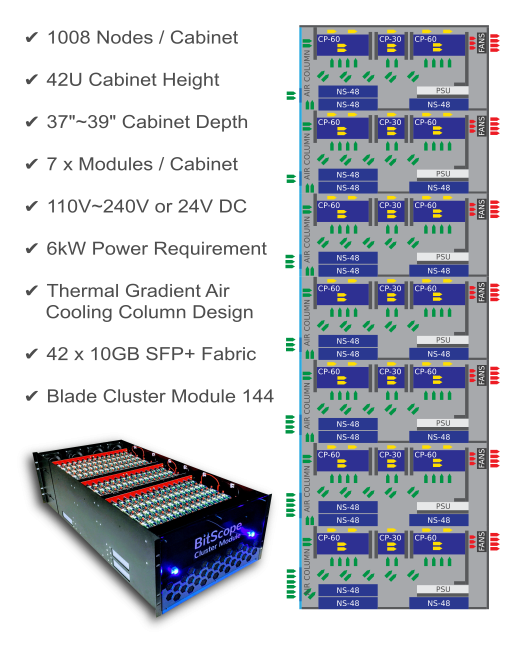
\includegraphics[width=0.5\textwidth]{images/rack-overview.png}
\caption{Rack placement of multiple Bitscope 144 cluster modules.}\label{F:pi-mod-2}
\end{figure}




\subsection{Links}\label{links}

Additional information about this form factor can be found at the
following links:

\URL{https://cluster.bitscope.com/solutions}
\URL{https://www.pcper.com/news/General-Tech/BitScope-Unveils-Raspberry-Pi-Cluster-2880-CPU-Cores-LANL-HPC-RD}
\URL{http://my.bitscope.com/store/}
\URL{http://my.bitscope.com/store/?p=view\&i=item+7}
\URL{http://www.newark.com/bitscope/bb04b/quattro-pi-board-raspberry-pi/dp/95Y0643}
\URL{http://linuxgizmos.com/rpi-expansion-boards-support-up-to-40-pi-clusters/}



\section{Build Your Own 5 Node Pi Cluster}\label{s:pi5}

To experiment with building an elementary cluster one does not need to
have a big budget. Such clusters are often dedicated to research tasks
and are bound into security protocols that do not allow direct
access. Instead it is possible to build such a cluster based on
Raspberry PI's yourself if you are willing to spend the money or if
you have access to PI's that you may loan from your department.

Table~\ref{T:picluster-partslist} lists one such possible parts list
that will allow you to build a cluster for up to 5 nodes. However make
sure to buy at least 3 Raspberry PI's with the appropriate memory. At
minimum we recommend you get the 32GB SD card. We do not recommend any
smaller as otherwise you will run out of memory. Additionally, you can
add memory and disks on te USB ports. If you attach a HDD, make sure
it has an external power supply and do not drive it from the USB power
as otherwise the PI becomes unstable.  A fan is at this time not yet
included.

Naturally it is possible to modify the parts list and adapt. If you
find better parts let us know. We have not included any case and you
are welcome to share your suggestions with the class. For a case we
are looking also for a good solution for a fan.

We suggest that when you build the cluster to do it on a table with a
large white paper or board, or a tablecloth and take pictures of the
various stages of the build so we can include it in this document.

Initially we just put rasbian as Operating system on the SD cards and
test out each PI. To do so you will naturally need an SD card writer
that you can hook up to your computer if it does not have one. As you
will have to potentially do this more than once it is not recommended
to buy an SD card with the OS on it. Buy the SD card writer instead so
you can redo the flashing of the card when needed. In addition to the
SD card you need a USB mouse and keyboard and a monitor or TV with
HDMI port.

Locate setup instructions and write  a tutorial in markdown that we
will include here once it is finished. The tutorial is to be managed
on github.

\TODO{Class: check the network hub if it is a good choice as the one we
  originally chose could not be brought in sufficient quantity.}

\begin{table}[htb]

\caption{Parts list for a Pi cluster, remember you need at least 3
  Raspberry Pis}\label{T:picluster-partslist}
\bigskip


\resizebox{\textwidth}{!}{%
\begin{tabular}{rp{13cm}p{1cm}}
  \hline
  Price   &  Description & URL          \\
  \hline
  \hline
  \$29.99 & 
            Anker 60W 6-Port USB Wall Charger, PowerPort 6 for iPhone 7 / 6s /
            Plus, iPad Pro / Air 2 / mini, Galaxy S7 / S6 / Edge /
            Plus, Note 5 / 4, LG, Nexus, HTC and More  
                         & 
                           \href{https://www.amazon.com/Anker-6-Port-Charger-PowerPort-iPhone/dp/B00P933OJC/ref=pd\_sim\_107\_70?\_encoding=UTF8\&psc=1\&refRID=B1S6V5G0CTJ9NH5G0CRT}{link}
  \\

  \$8.90  & 
            Cat 6 Ethernet Cable 1 ft White ( 6 Pack ) – Flat Internet Network
            Cable – Jadaol Cat 6 Computer Cable short - Cat6 Ethernet
            Patch Lan Cable With &
                                   \href{https://www.amazon.com/Cat-Ethernet-Cable-White-Pack/dp/B01IQWGI0O/ref=sr\_1\_1?s=electronics\&ie=UTF8\&qid=1513699717\&sr=1-1\&keywords=Cat+6+Ethernet+Cable+1+ft+White+\%28+6+Pack+\%29+\%E2\%80\%93+Flat+Internet+Network+Cable+\%E2\%80\%93+Jadaol+Cat+6+Computer+Cable+short+-+Cat6+Ethernet+Patch+Lan+Cable+With\%E2\%80\%A6}{link}  \\

  $^{(1)}$ \$19.99 &  D-link 8-Port Unmanaged Gigabit Switch
            (GO-SW-8G)   & 
                           \href{https://www.amazon.com/D-link-8-Port-Unmanaged-Gigabit-GO-SW-8G/dp/B008PC1MSO}{link}      \\


  \$10.49 &  SanDisk Ultra 32GB microSDHC UHS-I Card with
            Adapter, Grey/Red, Standard Packaging
            (SDSQUNC-032G-GN6MA)
                         & 
                           \href{https://www.amazon.com/SanDisk-microSDHC-Standard-Packaging-SDSQUNC-032G-GN6MA/dp/B010Q57T02/ref=sr\_1\_10?s=pc\&rps=1\&ie=UTF8\&qid=1498443283\&sr=1-10\&refinements=p\_85:2470955011,p\_n\_feature\_two\_browse-bin:6518304011,p\_n\_feature\_keywords\_two\_browse-bin:5947557011}{link}       \\

  \$8.59  & Short USB Cable, OKRAY 10 Pack Colorful Micro
            USB 2.0 Charging Data Sync Cable Cord for
            Samsung, Android Phone and Tablet, Nexus, HTC,
            Nokia, LG, Sony, Many Digital Cameras-0.66ft
            (7.87 Inch) & 
                          \href{https://www.amazon.com/OKRAY-Colorful-Charging-Samsung-Cameras-0-66ft/dp/B00R5GZJR6/ref=sr\_1\_6?s=pc\&ie=UTF8\&qid=1498447476\&sr=1-6\&keywords=micro+usb+cable+1ft}{link}         \\


  \$7.69    & 50 Pcs M2 x 20mm + 5mm Hex Hexagonal Threaded
              Spacer Support
                         & 
                           \href{https://www.amazon.com/20mm-Hexagonal-Threaded-Spacer-Support/dp/B00FH8AB8Q/ref=sr\_1\_9?s=industrial\&ie=UTF8\&qid=1513700337\&sr=1-9\&keywords=hex+spacers+m2+20mm}{link}
  \\

  \$7.99  & Easycargo 15 pcs Raspberry Pi Heatsink Aluminum
            + Copper + 3M 8810 thermal conductive adhesive
            tape for cooling cooler Raspberry Pi 3, Pi 2,
            Pi Model B+
                         & 
                           \href{https://www.amazon.com/Easycargo-Raspberry-Heatsink-Aluminum-conductive/dp/B07217N5LS/ref=sr\_1\_3?s=industrial\&ie=UTF8\&qid=1513700498\&sr=1-3\&keywords=raspberry+pi+3}{link}
  \\

  \$34.49 & Raspberry Pi 3 Model B Motherboard  (you need at least 3 of them)   & 
                                                                                  \href{https://www.amazon.com/Raspberry-Pi-RASPBERRYPI3-MODB-1GB-Model-Motherboard/dp/B01CD5VC92}{link}
  \\

 $^{(2)}$ \$59.99 & 1TB drive   & \href{http://wdlabs.wd.com/products/wd-pidrive-berryboot-edition/}{link}    \\

  \$15.19 & 64GB flash  & \href{https://www.wdc.com/products/wdlabs/wd-pidrive-foundation-edition.html\#WD3750LMCW}{link} \\

  \$6.99  & HDMI Cable, Rankie 2-Pack 6FT Latest Standard
            HDMI 2.0 HDTV Cable - Supports Ethernet, 3D, 4K
            and Audio Return (Black) - R1108
                         & 
                           \href{https://www.amazon.com/Cable-Rankie-2-Pack-Latest-Standard/dp/B00Z07XQ4A/ref=sr\_1\_6?s=wireless\&ie=UTF8\&qid=1513782649\&sr=1-6\&keywords=hdmi+cable+6ft}{link}         \\

  \$12.99  & AUKEY USB C Adapter, USB C to USB 3.0 Adapter
             Aluminum 2 Pack for Samsung Note 8 S8 S8+,
             Google Pixel 2 XL, MacBook Pro, Nexus 6P 5X, LG
             G5 V20 (Gray)
                         & 
                           \href{https://www.amazon.com/Cat-Ethernet-Cable-White-Pack/dp/B01IQWGI0O/ref=pd\_sim\_147\_2?\_encoding=UTF8\&psc=1\&refRID=FZZ7E36666EJPDTH7B6A}{link}     \\

\$19.19 & For Raspberry Pi 3 2 TFT LCD Display, kuman 3.5
   Inch 480x320 TFT Touch Screen Monitor for
   Raspberry Pi Model B B+ A+ A Module SPI
   Interface with Touch Pen SC06
     & 
\href{https://www.amazon.com/Raspberry-Display-kuman-480x320-Interface/dp/B01CNJVG8K/ref=sr\_1\_1?s=electronics\&ie=UTF8\&qid=1513783748\&sr=1-1\&keywords=pi+3+lcd+screen+3.5in}{link} \\
\hline
\end{tabular}
}
\smallskip

{\footnotesize (1) items were replaced with similar item}\\
{\footnotesize (2) item was not available}

\end{table}


\begin{exercise}
\label{E:cluster-pi}
In case you do not have access to multiple PIs conduct the Single Pi
experiment.
\end{exercise}

\section{Single Pi}


You have been presented in Section
\ref{S:cluster-case-with-cooling-5-pi} with a table that compares
tempreatures. Your task is to identify issues with the experiment and
the table.  Furthermore we like you to rerun a temperature experiment
in the entire class.

\TODO{Gregor: Add IoT section and PI configuration}

\begin{enumerate}
\item
  Get a PI3 modeL B, an HDMI cable, a power supply, a case. Such a
  configuration is listed in the IoT section. 
\item
  Buy or manufacture a case of your choice. You can use a 3d-printer
  if you have one available.
\item
  Conduct a temperature experiment.
\end{enumerate}

Discussion of these assignment is to be executed openly in
class. Points will be issued only once the class agrees upon an
experiment.

This exercise is not only to learn about the behaviour of the Pi, but
also about how to coordinate experiments with a large number of
students.


\begin{exercise}
  \label{E:Exercise.Pi.Single.1} What temperature measurement is
  missing from the table.
\end{exercise}

\begin{exercise}
\label{E:.Pi.Single.2} How would you create an experiment under \textit{load}.
\end{exercise}

\begin{exercise}
\label{E:.Pi.Single.3} How would you create an experiment to which all
  students in different classes could contribute their values? Can the
  cloud be used?
\end{exercise}

\begin{exercise}
\label{E:.Pi.Single.4} Collect the information from all class members
  using cloud services.
\end{exercise}

\begin{exercise}
  \label{E:.Pi.Single.5} Identify how to use the VPN server so you can
  use your Laptop instead of a TV or computer monitor. Write a
  tutorial.
\end{exercise}



\section{Small Pi Cluster}

In this set of exercises we will be building a small Raspberry Pi
cluster. All of you will have to do Exercise
\ref{Exercise.Pi.Cluster.Build}, as well as one of the tasks related
to Swarm, kubernetes or Spark.

It is important that you write down all steps very carefully as you
are expected to use the steps to develop an automated deployment. For
your cluster. Your tutorial will be tested by other groups and easy of
installation completness, and correctness will be evaluated.  Teams
that find issues and improve deployment tutorials will receive points.
TA's will also replicate these steps to identify a fair evaluation
without bias.


\begin{exercise}

\label{E:.Pi.Cluster.Build} Build groups of up to 5 people. Make a
  plan on what needs to be done to build the cluster and develop a
  schedule. Include in this plan (a) obtaining the material the
  hardware build, (b) the installation of the operating system (c) the
  testing of the system (d) familiarizing with the OS.
\end{exercise}

\begin{exercise}

  \label{E:.Pi.Cluster.DockerSwarm} Install a docker Swarm cluster on
  your PI. Develop a tutorial in markdown and mind
  plagiarism. Contribute your tutorial to this document to get
  acknowledged and credit. Work with others in class to coordinate a
  single tutorial.
\end{exercise}

\begin{exercise}

  \label{E:.Pi.Cluster.Kubernetes} Install a kubernetes cluster on
  your PI. Develop a tutorial in markdown and mind
  plagiarism. Contribute your tutorial to this document to get
  acknowledged and credit. Work with others in class to coordinate a
  single tutorial.
\end{exercise}
  
\begin{exercise}
  \label{E:.Pi.Cluster.Spark} Install a spark cluster on your
  PI. Develop a tutorial in markdown and mind plagiarism. Contribute
  your tutorial to this document to get acknowledged and credit. Work
  with others in class to coordinate a single tutorial.
\end{exercise}


\subsection{Virtual Raspberry Cluster}

It should also be possible to craete a virtual raspberry PI cluster
while for example using virtual box. This requires two steps. First
the deployment of a virtualized Raspberry PI. The following
information may be useful for this

\URL{http://dbakevlar.com/2015/08/emulating-a-raspberry-pi-on-virtualbox/}

The next step includes the deployment of multiple VMs emulating
Raspberrys. Naturally each should have its own name so you can
distinguish them. INstead of just using the GUI, it would be improtant
to find out how to start them from a commandline as a shell script as
well as tear them down.

Next you will need to make sure you can communicate from the PIs to
each other. This is naturally the same as on a real cluster

\begin{exercise}
provide a tutorial 
\end{exercise}

This can be chosen as part of your project, but you need to develop a
cloudmesh command for managing the cluster. THis includes starting and
stoping as well as checkpointing the cluster from a cloudmesh
command. Furthermore you need to benchmark it and identify how to do
this and contrast this to other clusters that you may start or have
access to. Please get in contact with Gregor. THis prject is reserverd
for online students, as residential students will have access to real
Rasperry PI hardware.
